\section{Statistical Inference}

\begin{frame}{Statistical Inference}

    \textbf{Statistical inference is the process of deducing the population characteristics based on the sample.}
    
    Consider the following:
    
    \begin{columns}
        \begin{column}{0.5\textwidth}
            {\scriptsize \begin{itemize}
                \item Is the sample mean and SD the true population mean and SD?
                \item What is the underlying distribution?
                \item Does the sample distribution represent well the population?
                \item How likely is it to observe value $x$?
                \item What, most likely, the future observations will be?
            \end{itemize}}
        \end{column}
        \begin{column}{0.5\textwidth}
            \begin{figure}
                \includegraphics[width=\textwidth]{gfx/random_sampling}
            \end{figure}
        \end{column}
    \end{columns}

\end{frame}

\begin{frame}{Point Estimate}

    A \textbf{point estimate} is the ``best guess" for a population parameter based on a sample.
    
    \begin{example}
        \medskip
        Point estimates for the mean and SD of a population following a normal distribution $\mathcal{N}(\mu = 0, \sigma = 10)$ depending on the sample size:
        \only<1>{
            \includegraphics[width=\linewidth]{R/plots/point-estimate-vs-sample-size1}
        }
        \only<2>{
            \includegraphics[width=\linewidth]{R/plots/point-estimate-vs-sample-size2}
        }
    \end{example}

\end{frame}

\begin{frame}{Standard Error of the Mean}

    Let's assume we have a population of 1 million individuals following the normal distribution $\mathcal{N}(\mu = 5, \sigma = 3)$. This is the true histogram of the population:

    \includegraphics[width=\linewidth]{R/plots/se-population}

\end{frame}

\begin{frame}{Standard Error of the Mean}

    We draw 1000 independent samples of size 50, and for each sample calculate the mean. This is the distribution of the means:
    
    \begin{figure}
        \includegraphics[width=\linewidth]{R/plots/se-sampling-distribution-50}
    \end{figure}
    
\end{frame}

\begin{frame}[t]{Standard Error of the Mean}

    The \textbf{sampling distribution} of the mean depends on the number of samples and the sample size:

        \only<1>{
            \includegraphics[width=\linewidth]{R/plots/se-sampling-distribution-10-100-1000}
        }
        \only<2>{
            \includegraphics[width=\linewidth]{R/plots/se-sampling-distribution-boxplot}
            The obtained means are similar (5.12, 4.93, 4.99), but our level of confidence increases with the increasing sample size.
        }
%        \only<3>{
%            \begin{itemize}
%                \item the distribution becomes more ``normal" with more samples
%                \item the distribution becomes more dense (narrow) with larger samples
%            \end{itemize}
%        }
    

\end{frame}

\begin{frame}{Central Limit Theorem}

    \begin{block}{Central Limit Theorem (classical definition)}
        \medskip
        The sum of independent and identically distributed random variables tends toward a normal distribution.
    \end{block}

    \medskip
    \begin{block}{Central Limit Theorem (informal description w.r.t. the mean)}
        \medskip
        The sampling distribution of the mean $\bar{x}$ is approximately normal, even if $X$ is not normally distributed. The approximation improves with larger samples.
    \end{block}

\end{frame}

\begin{frame}{Examining the Central Limit Theorem}

    \begin{figure}
        \includegraphics[width=\linewidth]{R/plots/central-limit-theorem}
    \end{figure}

\end{frame}

\begin{frame}{Standard Error of the Mean}

    The \textbf{standard error of the mean ($SE_{\bar{x}}$)} is the standard deviation of the sampling distribution of the mean:
    
    \begin{equation}
    SE_{\bar{x}} = \frac{\sigma}{\sqrt{n}} \approx \frac{s}{\sqrt{n}}
    \end{equation}
    
    where:\\
    $\sigma$ -- population standard deviation (often unknown),\\
    $s$ -- sample standard deviation,\\
    $n$ -- sample size.
    \vspace{14pt}
    
    {\tiny
        The equation is valid for samples with independent observations.\\
        We can assume that observations are independent if the sample consists of less than 10\% of the population.}

\end{frame}

\begin{frame}{Why is it useful?}
    
    \begin{example}
        \medskip
        Discuss in groups how could you use the Central Limit Theorem, including the equation for $SE_{\bar{x}}$, in:
        \begin{itemize}
            \item guessing the range in which the population mean is most likely located,
            \item assessing the probability of observing certain mean from a random sample.
        \end{itemize}
    \end{example}

\end{frame}


\begin{frame}[fragile]{Standardized Random Variable (Z-score)}

    \begin{example}
        \medskip
        {\small
        \begin{verbatim}
        N = 1000
        X <- rnorm(N, mean = 10, sd = 2)
        Z <- (X - mean(X)) / sd(X)
        plot(density(Z))
        xgrid <- seq(-4, 4, by = 0.1, lty=1)
        lines(xgrid, dnorm(xgrid), lty=2)
        \end{verbatim}}
        \begin{itemize}
            \item Why $Z$ has mean equal to 0 and standard deviation\\equal to 1?
            \item How does the distribution of $Z$ depend on the sample size $N$?
        \end{itemize}
    \end{example}

\end{frame}

\begin{frame}{Standardized Random Variable (Z-score)}
    \begin{figure}
        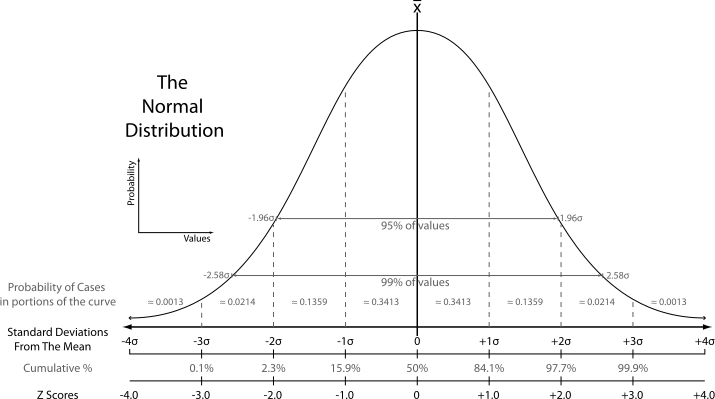
\includegraphics[width=0.85\linewidth]{gfx/web/The_Normal_Distribution}
    \end{figure}
    
    \begin{equation}
    Z = \frac{X - \mu}{\sigma}
    \end{equation}
    
    {\tiny Image based on: \url{https://commons.wikimedia.org/wiki/File:The_Normal_Distribution.svg}}
\end{frame}

\begin{frame}{Standardized Sampling Distribution of the Mean}

    Let $\bar{x}$ be a sampling distribution of the mean from a population $X \sim \mathcal{N}(\mu, \sigma)$. The standardized version of $\bar{x}$ is:
    \begin{equation}
    Z = \frac{\bar{x} - \mu}{\sigma / \sqrt{n}} = \frac{\bar{x} - \mu}{SE_{\bar{x}}}
    \end{equation}
    
    $Z$ converges in distribution to $\mathcal{N}(\mu = 0, \sigma = 1)$ with the increasing number of samples. The sample size $n$ does not affect the distribution of $Z$ (because it's normalized).
    
    \begin{figure}
        \includegraphics[width=0.85\linewidth]{R/plots/standardization}
    \end{figure}

\end{frame}

\begin{frame}{Confidence Intervals}

    A plausible range of values for the population parameter (e.g. mean) is called a \textbf{confidence interval (CI)}. It's calculated using the point estimate and the standard error. The $c$\% confidence interval for the mean is given by:

    \begin{equation}
    \text{point estimate} \pm z^* \times SE_{\bar{x}}
    \end{equation}
    
    \begin{table}
        \begin{tabular}{c | c c c}
            $c$ & 90\% & 95\% & 99\% \\ \hline
            $z^*$ & 1.6 & 2.0 & 2.6 \\
        \end{tabular}
    \end{table}
    
    $z^* \times SE_{\bar{x}}$ is called \textbf{the margin of error}.
    
    {\tiny Note: The given values for $z^*$ are approximate. You can calculate the exact ones for any $c$\% using \texttt{qnorm()}.}

\end{frame}

\begin{frame}{Confidence Intervals}

    An example of 90\% CI calculated for 30 samples (dashed line -- true mean):

    \includegraphics[width=\linewidth]{R/plots/CI}
    \only<1>{If the sampling is repeated many times, in 90\% of cases the CI will encompass the true mean.}
    \only<2>{\sout{{\small There is a 90\% probability that the true mean lies within a specific CI}} \\$\rightarrow$ {\small NOT TRUE (the true mean is not a random variable)}}

\end{frame}

\begin{frame}{Confidence Intervals}

     \begin{example}
         \medskip
         Calculate a 95\% CI for the mean based on the following observations $^{*}$:\\
         14.6, 9.0, 11.5, 17.6, 13.2
         
         Use the standard normal distribution. Consider two cases:
         \begin{enumerate}
             \item Estimate $\sigma$ using the sample standard deviation $s$ $^{**}$.
             \item Use the true standard deviation $\sigma = 5$.
         \end{enumerate}
     \end{example}
    \bigskip

    \tiny * The sample was generated with the following command: \texttt{rnorm(5, mean = 10, sd = 5)}\\
    \tiny ** Read the docs: \texttt{?sd}

\end{frame}

\begin{frame}{Confidence Intervals When $\sigma$ is Unknown}

    In the case when we don't know the population standard deviation $\sigma$ and the sample size is small ($< 30$), we can't use the normal distribution. Instead, we use the $t$-distribution:
    \begin{equation}
    \text{point estimate} \pm t_{df}^* \times SE_{\bar{x}}
    \end{equation}   
    where the degrees of freedom $df = n - 1$, and $n$ is the sample size. The standard error $SE_{\bar{x}}$ is calculated as previously.

\end{frame}

\begin{frame}{t-Distribution (Repetition)}
    
    If the sample size is small ($n < 30$) and the population standard deviation is unknown, we often use the t-distribution instead of the normal distribution. t-distribution depends only on the number of degrees of freedom $df = n - 1$. For $df \ge 30$ it's almost indistinguishable from the standard normal distribution.
    
    \includegraphics[width=\linewidth]{R/plots/t_distribution}
    {\tiny R commands: \texttt{dt}, \texttt{pt}, \texttt{qt}, \texttt{rt}}

\end{frame}

\begin{frame}{Confidence Intervals}
    \begin{example}
        \medskip
        Calculate the exact $z^*$, $t_{df}^*$ values for the following confidence levels: 90\%, 95\%, 99\%, 99.9\%. Use the standard normal distribution and the t-distribution. Assume the sample size $s = 5$.
    \end{example}

    \begin{tabular}{c | c c c c }
        $c$\%       & 90\% & 95\% & 99\% & 99.9\% \\
        \hline
        $z^*$       &      &      &      &         \\
        \hline
        $t^*_{df}$  &      &      &      &         \\
    \end{tabular}
    \bigskip

    {\tiny Hint: Use \texttt{qnorm(p)}, \texttt{qt(p, df)}}
\end{frame}

\begin{frame}{Confidence Intervals Based on the t-Distribution}
    \begin{example}
        \medskip
        Calculate 95\% and 99\% CIs for the mean based on the following observations:\\
        14.6, 9.0, 11.5, 17.6, 13.2
        
        Use the $t$-distribution.
    \end{example}
    \bigskip
    
    {\tiny Hint: Use \texttt{qt(p, df)}}
\end{frame}

\begin{frame}{Confidence Intervals: Practical Example}

    \begin{example}
        \medskip
        Using the previously collected data about the height of SDU students (\url{http://bit.ly/sta2018-height}), calculate 95\% and 99\% CIs for the mean height.
        
        Compare the CIs based on the t-distribution and the normal distribution (assume that the sample standard deviation is the population standard deviation). Interpret the results.
    \end{example}

\end{frame}

\begin{frame}{Repetition}

    \begin{example}
        \medskip
        True or false?
        \begin{itemize}
            \item Confidence intervals describe the probability that the true mean lies within the interval.
            \item 99\% confidence interval is wider than a 95\% confidence interval.
            \item When a sample follows the normal distribution, we should use the normal distribution to calculate the confidence interval.
            \item Confidence interval gets narrower with the increasing size of the samples.
            \item Confidence interval gets narrower with the increasing number of samples.
        \end{itemize}
    \end{example}

\end{frame}

\begin{frame}{Hypothesis Testing}

    \textbf{Hypothesis testing} is a statistical technique for comparing two exclusive hypotheses: a null hypothesis $H_0$ and an alternative hypothesis $H_A$. E.g.:
    \begin{itemize}
        \item $H_0$: the new drug and the old drug are equally effective
        \item $H_A$: the new drug is better than the old
    \end{itemize}

    The null hypothesis $H_0$ often represents a skeptical perspective or a claim to be tested. The null hypothesis $H_0$ is not rejected unless the evidence in favor of the alternative hypothesis $H_A$ is strong.

\end{frame}

\begin{frame}{Hypothesis Testing}

    Hypotheses can be described mathematically, e.g.:
    \medskip

    \begin{math}
        \left.
            \begin{array}{l}
                H_0: \mu = x\\
                H_A: \mu \ne x            
            \end{array}
        \right\}
        \text{double-sided test}
    \end{math}
    \medskip
    
    or
    \medskip
    
    \begin{math}
        \left.
            \begin{array}{l}
                H_0: \mu = x\\
                H_A: \mu > x            
            \end{array}
        \right\}
        \text{single-sided test}
    \end{math}

\end{frame}

\begin{frame}{Hypothesis Testing}

    Hypotheses can be tested with:
    \begin{enumerate}
        \item Confidence intervals (suitable for double-sided tests)
        \item p-values (suitable for both single- and double-sided tests)
    \end{enumerate}

    \begin{example}
        \medskip
        Why confidence intervals are not suitable for single-sided tests?\\
        Give an example of a single-sided test.
    \end{example}

\end{frame}

\begin{frame}{Hypothesis Testing Using Confidence Intervals}

\begin{enumerate}
    \item Formulate $H_0$, $H_A$, and the confidence level (90\%, 95\%, 99\%)
    \item Assume the model (normal distribution or $t$-distribution)
    \item Find $z^*$ or $t_{df}^*$
    \item Calculate the confidence interval:
    \begin{itemize}
        \item normal distribution $\rightarrow \bar{x} \pm z^* \times SE_{\bar{x}}$\\
        \item $t$-distribution: $\rightarrow \bar{x} \pm t_{df}^* \times SE_{\bar{x}}$
    \end{itemize}
    \item Reject $H_0$ if the mean you are comparing to $\bar{x}_2$ (or population mean $\mu$) lies outside the confidence interval
\end{enumerate}

\end{frame}

\begin{frame}{Hypothesis Testing Using p-Value}

    \begin{enumerate}
        \item Formulate $H_0$, $H_A$, and the significance level $\alpha$ (e.g. 0.05)
        \item Assume the model (normal distribution or $t$-distribution)
        \item Calculate the test statistic ($Z$-score or $t$-score)
        \item Calculate the p-value
        \item Reject $H_0$ if p-value $< \alpha$
    \end{enumerate}
    \begin{figure}
        \includegraphics[width=\linewidth]{R/plots/hypothesis_testing}
    \end{figure}

\end{frame}

\begin{frame}{Hypothesis Testing: Factory Example \#1}
     \begin{example}
         \medskip
         A factory claims that the average lifetime of the sensors it produces is 3 years. A random sample of 100 sensors was taken and they worked for 2.8 years on average with the standard deviation of 0.9 years.
         
         Construct the null and alternative hypotheses and evaluate whether there is a sufficient evidence to reject the null hypothesis.
         
         Use both (a) confidence intervals and (b) p-values.
     \end{example}
\end{frame}

\begin{frame}{Factory Example \#1: Hypotheses}

    The hypotheses could be as follows:

    \begin{math}
        \begin{array}{l l}
            H_0: &\mu = 3\\
            H_A: &\mu \ne 3
        \end{array}
    \end{math}
    \medskip
    
    Alternatively, if we expect that the actual sensor lifetime is shorter than 3 years:
    
    \begin{math}
        \begin{array}{l l}
            H_0: &\mu = 3\\
            H_A: &\mu < 3
        \end{array}
    \end{math}
    
\end{frame}

\begin{shownto}{teacher}
    \begin{frame}{Factory Example \#1: Confidence Intervals}
    
        \begin{enumerate}
            \item The sample is sufficiently large to use the normal model.
            \item The population standard deviation can be approximated with the sample standard deviation.
            \item The sample likely consists of less than 10\% of the population, so we can assume that the observations are independent.
            \item Let's assume a 95\% confidence interval $\rightarrow z^* = 2$.
        \end{enumerate}
    
        \begin{equation*}
        3 \pm z^* \times SE_{\bar{x}} \rightarrow
        3 \pm 2 \times \frac{s}{\sqrt{n}} \rightarrow
        3 \pm 2 \times \frac{0.9}{\sqrt{100}} \rightarrow
        3 \pm 0.18
        \end{equation*}
        \medskip
    
        The sample mean $\bar{x} = 2.8$ is outside the confidence interval, so we have \textbf{sufficient evidence to reject the null hypothesis}.
        
    \end{frame}
    
    \begin{frame}{Factory Example \#1: p-Values}
        Let's keep assumptions 1-3 from the previous slide. We'll use the significance level $\alpha = 0.05$.
        
        \begin{figure}
            \includegraphics[width=\linewidth]{R/plots/factory-1-p-value}
        \end{figure}
    
        Single-sided test ($H_A: \mu < 3$):
        \begin{equation*}
        p\text{-value} = 0.013 < \alpha = 0.05 \rightarrow \text{Reject } H_0
        \end{equation*}
    
        Double-sided test ($H_A: \mu \ne 3$):
        \begin{equation*}
        p\text{-value} = 0.026 < \alpha = 0.05 \rightarrow \text{Reject } H_0
        \end{equation*}
    
    \end{frame}
\end{shownto}

\begin{frame}{Hypothesis Testing: Factory Example \#2}
    \begin{example}
        \medskip
        %TODO: ADD SLIDE WITH CALCULATION OF SE FOR TWO SAMPLES!!!
        A factory produces 100 thousands sensors per year. A sample of 10 sensors was taken for extensive field tests and it turned out the sensors worked with a sufficient accuracy for 20 months on average, with a standard deviation of 5 months. After that time they needed a recalibration.
        
        After introducing stricter quality assurance (QA) procedures in the factory, another sample of 10 sensors was taken and this time the average time of accurate work was 27 months with a standard deviation of 6 months.
        
        Determine whether the results give a statistically significant evidence that the new QA procedures improved the average sensor lifetime. Perform the test based on p-values.
    \end{example}
\end{frame}

\begin{frame}{Standard Error For The Difference of Two Means}
    If we test a hypothesis in a form\\
    $H_0$: $\mu_1 - \mu_2 = 0$,\\
    $H_A$: $\mu_1 - \mu_2 \ne 0$,\\
    where $\mu_1$, $\mu_2$ are the means of \emph{two different populations}, we need to calculate the standard error based on two samples:
    \begin{equation}
    SE_{\bar{x}_1 - \bar{x}_2} = \sqrt{\frac{\sigma_1^2}{n_1} + \frac{\sigma_2^2}{n_2}} \approx \sqrt{\frac{s_1^2}{n_1} + \frac{s_2^2}{n_2}}.
    \end{equation}
    
    If we use the $t$-distribution, we can assume that $df = \min \left(n_1 - 1; n_2 - 1\right)$.
\end{frame}

\begin{shownto}{teacher}
    \begin{frame}{Factory Example \#2: p-Values}
    $H_0 : \bar{x}_2 - \bar{x}_1 = 0$\\    
    $H_A : \bar{x}_2 - \bar{x}_1 > 0$
    
    $df = \min \left( 10 - 1; 10 - 1 \right) = 9$
    
    $SE_{\bar{x}_2 - \bar{x}_1} = \sqrt{\frac{5^2}{10} + \frac{6^2}{10}} = 2.47$
    
    $Z = \frac{(27-20) - 0}{2.47} = 2.83$
    
    p-value $= P(Z \ge 2.83) = 0.01 \quad$ {\small/\texttt{1-pt(2.83, df=9)}/}
    
    If we assume $\alpha = 0.05$, p-value $< \alpha$ and we reject $H_0$. But what would you do if $\alpha = 0.01$?

    \end{frame}
\end{shownto}
